% z'=y, y=u, u=1 before t=.5 and2 afterward. z=t or2t-.5.
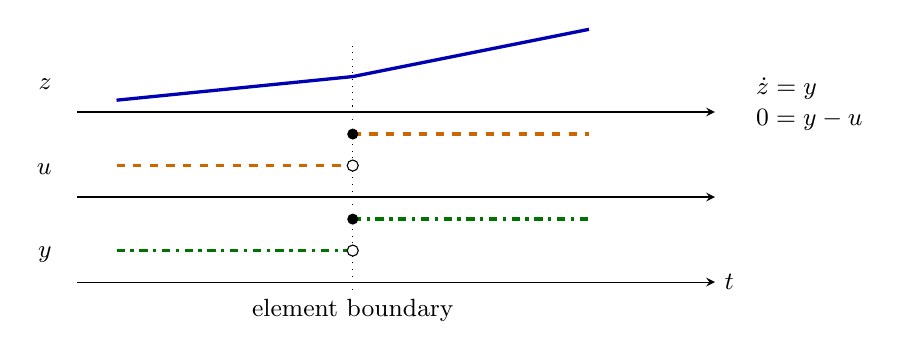
\begin{tikzpicture}[>=stealth,x=1cm,y=1cm,font=\small]
\foreach \row/\name in {0/z,1/u,2/y}{
\begin{scope}[shift={(0,-1.08*\row)}]
\draw[->,black](.5,0)--(8.6,0);
\node[anchor=east]at(.3,.35){$\name$};
\draw[dotted,black](4,-.1)--(4,.9);
\end{scope}}
\draw[blue!70!black,very thick](1,.15)--(4,.45)--(7,1.05);
\draw[orange!80!black,very thick,dashed](1,-.68)--(4,-.68);
\draw[orange!80!black,very thick,dashed](4,-.28)--(7,-.28);
\draw[green!45!black,very thick,dash dot](1,-1.76)--(4,-1.76);
\draw[green!45!black,very thick,dash dot](4,-1.36)--(7,-1.36);
\foreach \y in {-.68,-1.76}{\draw[fill=white](4,\y)circle(2pt);}
\foreach \y in {-.28,-1.36}{\fill(4,\y)circle(2pt);}
\node[below]at(4,-2.25){element boundary};\node[right]at(8.6,-2.16){$t$};
\node[align=left,anchor=west]at(9,.1){$\dot z=y$\\$0=y-u$};
\end{tikzpicture}
